\documentclass[a4paper,10pt]{ltjsarticle}
\usepackage[margin=18mm]{geometry}
\usepackage{amsmath,amssymb,graphicx,booktabs,float}
\usepackage[hidelinks]{hyperref}
\setlength{\parindent}{1em}
\title{傾斜平面間の角スペクトル直接変換\\理論整理と45度Originalホログラムからの変換実験}
\author{研究実験報告}
\date{2026年11月19日}
\begin{document}
\maketitle\small
\section{資料に基づく変換理論}
本節は提供資料「P1-P2直接変換」のPDFおよびWordに記載された式を整理する。
特に3ページ目の\textit{Direct Angular Spectrum Transformation between Tilted Planes}を対象とする。
資料の行列成分の配置と最終的な周波数座標式を採用し、途中の転置表記の揺れは再掲しない。

\subsection{座標系と角スペクトル}
基準面を$P_0$、2つの平面を$P_1,P_2$とし、資料に従い
\begin{equation}
 \boldsymbol r_1=R_1\boldsymbol r_0,\quad
 \boldsymbol r_2=R_2\boldsymbol r_0,\quad
 R_1=\begin{bmatrix}a_1&a_4&a_7\\a_2&a_5&a_8\\a_3&a_6&a_9\end{bmatrix},\quad
 R_2=\begin{bmatrix}b_1&b_4&b_7\\b_2&b_5&b_8\\b_3&b_6&b_9\end{bmatrix}
\end{equation}
と定義する。波長を$\lambda$とし、平面$i$の複素振幅とスペクトルを
\begin{equation}
 h_i(x_i,y_i)=\iint F_i(u_i,v_i)e^{\mathrm i2\pi(u_ix_i+v_iy_i)}\,du_i\,dv_i,
 \qquad w_i=\sqrt{\lambda^{-2}-u_i^2-v_i^2}
\end{equation}
で表す。以下では平方根が実数となる伝搬成分を扱う。

\subsection{$P_1$から$P_0$への対応}
資料では、基準面でのキャリア
$C_0=\exp[\mathrm i2\pi(a_3x_0+a_6y_0)/\lambda]$により、
$u'_0=u_0+a_3/\lambda$, $v'_0=v_0+a_6/\lambda$という周波数シフトが生じる。
波数ベクトルの座標対応を用いると、
\begin{align}
 u_0&=a_1u_1+a_2v_1+a_3w_1-a_3/\lambda,\\
 v_0&=a_4u_1+a_5v_1+a_6w_1-a_6/\lambda
\end{align}
となる。

\subsection{$P_0$から$P_2$への対応と直接変換}
もう一方の面のキャリアに対応するシフトを加えると、資料の式は
\begin{align}
 u_2&=b_1(u_0+b_3/\lambda)+b_4(v_0+b_6/\lambda)+b_7w'_0,\\
 v_2&=b_2(u_0+b_3/\lambda)+b_5(v_0+b_6/\lambda)+b_8w'_0,\\
 w'_0&=\sqrt{\lambda^{-2}-(u_0+b_3/\lambda)^2-(v_0+b_6/\lambda)^2}
\end{align}
となる。$A=a_1u_1+a_2v_1+a_3w_1-a_3/\lambda$、
$B=a_4u_1+a_5v_1+a_6w_1-a_6/\lambda$と置くと、合成した直接変換は
\begin{align}
 u_2&=b_1(A+b_3/\lambda)+b_4(B+b_6/\lambda)
       +b_7\sqrt{\lambda^{-2}-(A+b_3/\lambda)^2-(B+b_6/\lambda)^2},\\
 v_2&=b_2(A+b_3/\lambda)+b_5(B+b_6/\lambda)
       +b_8\sqrt{\lambda^{-2}-(A+b_3/\lambda)^2-(B+b_6/\lambda)^2}
\end{align}
である。資料のスペクトル変換は
\begin{equation}
 F_1(u_1,v_1)=J F_2\bigl(u_2(u_1,v_1),v_2(u_1,v_1)\bigr),\qquad
 J=\left|\det\frac{\partial(u_2,v_2)}{\partial(u_1,v_1)}\right|
\end{equation}
となる。これは出力格子から入力スペクトルの参照座標を求める形である。
面の名前と補間時の入出力の割当てを区別する必要がある。

\clearpage
\section{今回の実装}
\subsection{$R_1=I$のときの直接変換と$P_0\to P_2$の等価性}
今回の研究段階では$R_1=I$とする。このとき
\begin{equation}
 a_1=a_5=a_9=1,\qquad
 a_2=a_3=a_4=a_6=a_7=a_8=0
\end{equation}
なので、最初の変換は$u_0=u_1$, $v_0=v_1$となる。
これを直接変換式に代入すると、$(u_1,v_1)$と$(u_2,v_2)$の関係は
\begin{align}
 u_2&=b_1\left(u_1+\frac{b_3}{\lambda}\right)
      +b_4\left(v_1+\frac{b_6}{\lambda}\right)+b_7\widetilde w,\\
 v_2&=b_2\left(u_1+\frac{b_3}{\lambda}\right)
      +b_5\left(v_1+\frac{b_6}{\lambda}\right)+b_8\widetilde w,\\
 \widetilde w&=\sqrt{\lambda^{-2}
             -\left(u_1+\frac{b_3}{\lambda}\right)^2
             -\left(v_1+\frac{b_6}{\lambda}\right)^2}
\end{align}
となる。これは前節の$P_0\to P_2$の式で$u_0,v_0$を$u_1,v_1$と
書き換えたものに等しい。すなわち、同一の原点を用いる資料の回転モデルでは、
$P_1$と$P_0$の座標系が一致するため、$P_1\to P_2$の周波数座標写像は
$P_0\to P_2$と等価になる。連鎖律からも
\begin{equation}
 \frac{\partial(u_2,v_2)}{\partial(u_1,v_1)}
 =\frac{\partial(u_2,v_2)}{\partial(u_0,v_0)}
  \underbrace{\frac{\partial(u_0,v_0)}{\partial(u_1,v_1)}}_{I_2}
 =\frac{\partial(u_2,v_2)}{\partial(u_0,v_0)}
\end{equation}
であり、ヤコビアン補正も等しい。
この等価性は周波数座標写像について述べたもので、入力物体の傾斜角を推定する処理ではない。
物体回転や別途加えた伝搬の効果まで、この代入だけで同一とするものではない。

\subsection{y軸回転への限定}
残る行列を
\begin{equation}
 R_2=R_y(\delta)=\begin{bmatrix}c&0&s\\0&1&0\\-s&0&c\end{bmatrix},
 \quad c=\cos\delta,\ s=\sin\delta
\end{equation}
とすると、出力格子$(U,V)$から入力スペクトルを参照する座標は
\begin{align}
 U_{\rm phys}&=U-s/\lambda,\quad V_{\rm phys}=V,\\
 W_{\rm phys}&=\sqrt{\lambda^{-2}-U_{\rm phys}^2-V_{\rm phys}^2},\\
 \alpha&=cU_{\rm phys}+sW_{\rm phys},\qquad \beta=V_{\rm phys}
\end{align}
となる。平方根の微分は$\partial W_{\rm phys}/\partial U=-U_{\rm phys}/W_{\rm phys}$なので、
\begin{equation}
 J=\left|c-s\frac{U_{\rm phys}}{W_{\rm phys}}\right|
\end{equation}
を用いる。元コードの微分項にあった加算符号は減算に修正した。

\subsection{生成手順と条件}
入力は\texttt{original/npy/090\_+45.npy}であり、すべての出力で同じOriginal 45度を用いた。
相対角$\delta=-1,-2,\ldots,-45$度の45条件を独立に計算し、
比較先の公称物体角度を$\theta=45+\delta$度とした。
直前の結果を入力にする連続変換ではない。
公称角度と幾何学的な回転方向の一致は、本実験だけで独立に確定したものではない。

\begin{table}[H]\centering
\caption{生成条件（既存のOriginal生成コードに合わせた数値単位）}
\begin{tabular}{ll}\toprule
項目&設定\\\midrule
入力・出力画素数&$512\times512$\\
ゼロパディング後&$1024\times1024$\\
標本間隔&$4.5\times10^{-3}$\\
波長&$530\times10^{-6}$\\
回転前・後の伝搬距離&$+2$, $-2$\\
補間&\texttt{RegularGridInterpolator}, \texttt{method='cubic'}\\
補間範囲外&0\\\bottomrule
\end{tabular}\end{table}
伝搬関数$H_z=\exp(\mathrm i2\pi z\sqrt{\lambda^{-2}-U^2-V^2})$を用い、
入力をパディングしてFFTし、$H_{+2}$で伝搬したスペクトルを補間・ヤコビアン補正する。
その後$H_{-2}$を乗じ、逆FFTと中央切出しを行って複素ホログラムを保存した。
生成スクリプトは\texttt{generate\_from\_original45.py}である。

\subsection{評価方法}
既存の\texttt{PSNR.py}の\texttt{calculate\_psnr}と\texttt{calculate\_ssim}を使用した。
評価対象は再構成像ではなく、保存されたホログラムの振幅である。
Originalの振幅を$A$、生成結果の振幅を$B$とし、
\begin{equation}
 \widehat A=\frac{A-\min A}{\max A-\min A},\qquad
 \widehat B=\frac{B-\min A}{\max A-\min A}
\end{equation}
とする。生成結果もOriginalの範囲で正規化し、クリッピングせず、
両指標の\texttt{data\_range}を1とした。
PSNRは$10\log_{10}(1/\operatorname{MSE}(\widehat A,\widehat B))$、
SSIMは既存関数の既定の局所窓設定により計算する。
位相の一致度は今回の評価対象に含まれない。

\clearpage
\section{実装結果}
\begin{figure}[H]\centering
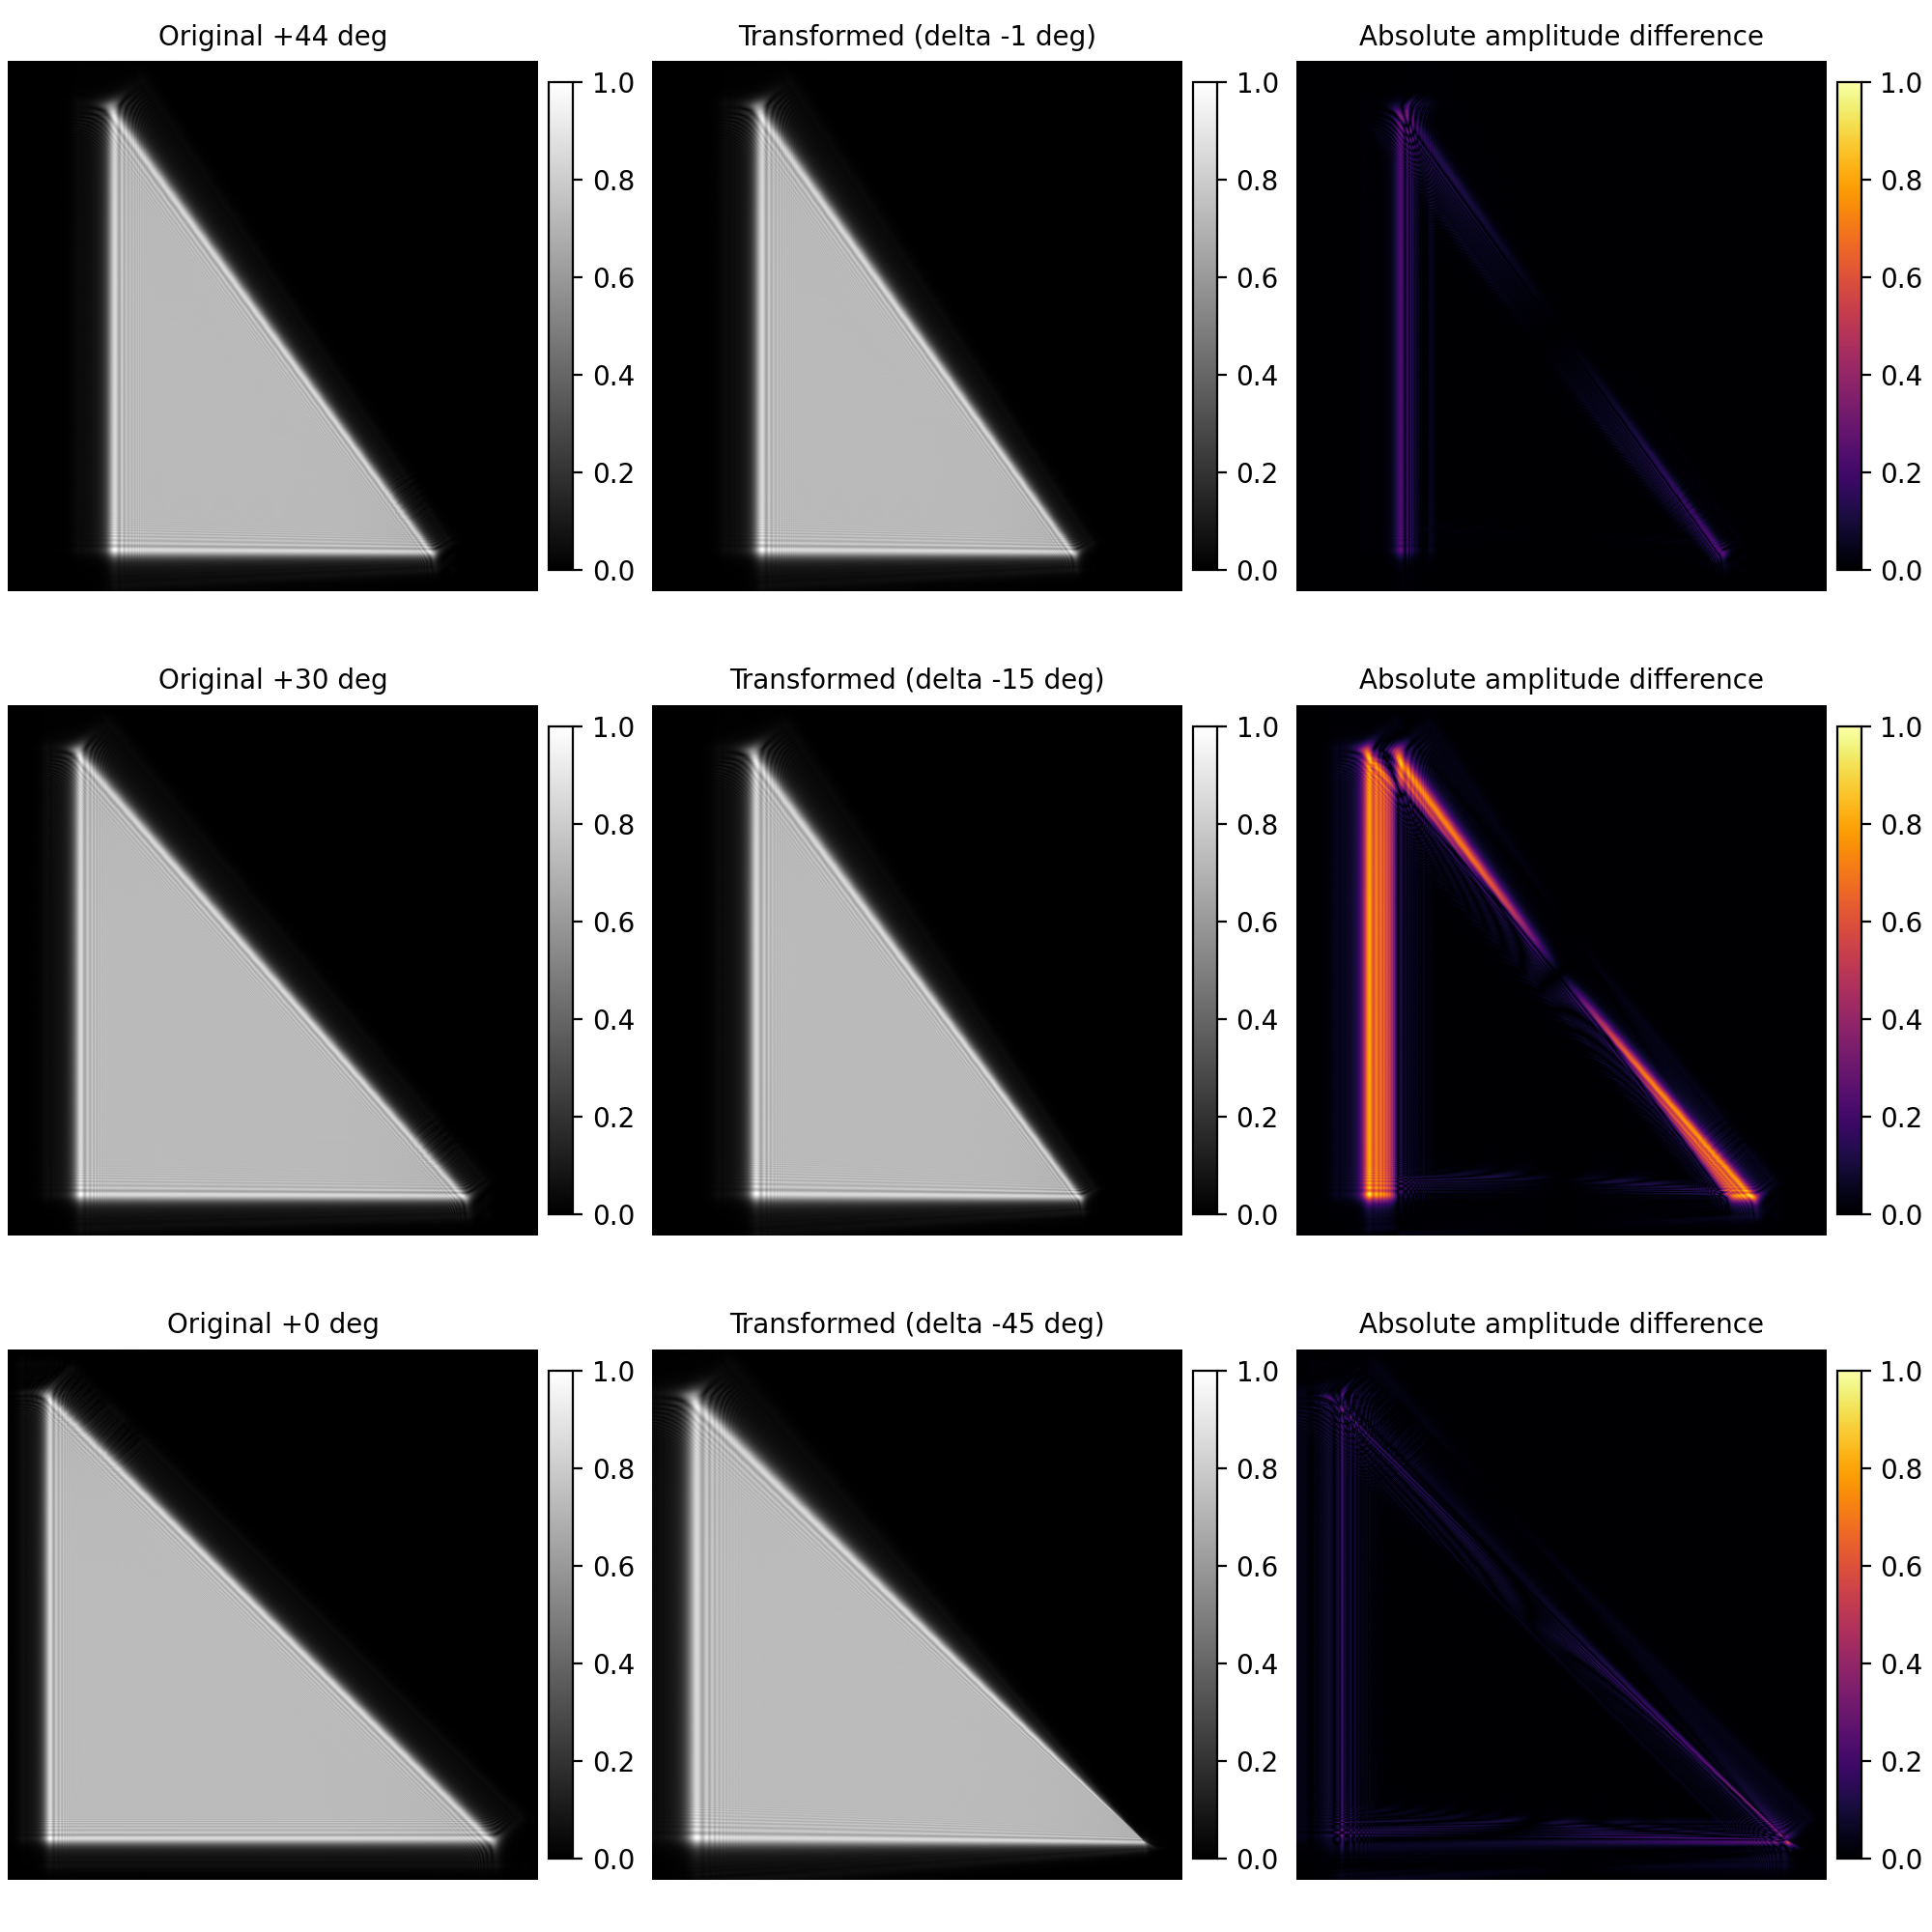
\includegraphics[width=.85\linewidth]{figures/amplitude_comparison.png}
\caption{上から公称44度（相対$-1$度）、30度（$-15$度）、0度（$-45$度）。
左はOriginal振幅、中央は変換後振幅、右は正規化振幅差の絶対値。
各行は対応するOriginalの最小値・最大値で正規化し、表示範囲を0から1に統一した。
再構成像ではなくホログラム面の振幅を示す。}
\end{figure}
\begin{table}[H]\centering
\caption{代表条件の振幅評価値}
\begin{tabular}{rrrr}\toprule
相対角[度]&比較先Original[度]&PSNR [dB]&SSIM\\\midrule
-1 & +44 & 29.5302 & 0.9132 \\
-15 & +30 & 15.5781 & 0.7306 \\
-45 & +0 & 29.1934 & 0.8276 \\
\bottomrule\end{tabular}\end{table}
代表画像と数値の双方により、角度によってOriginalとの差が変化することを確認した。
すべての出力は有限値を持つ$512\times512$の複素配列である。

\clearpage
\subsection{全45条件の評価と考察}
\begin{figure}[H]\centering
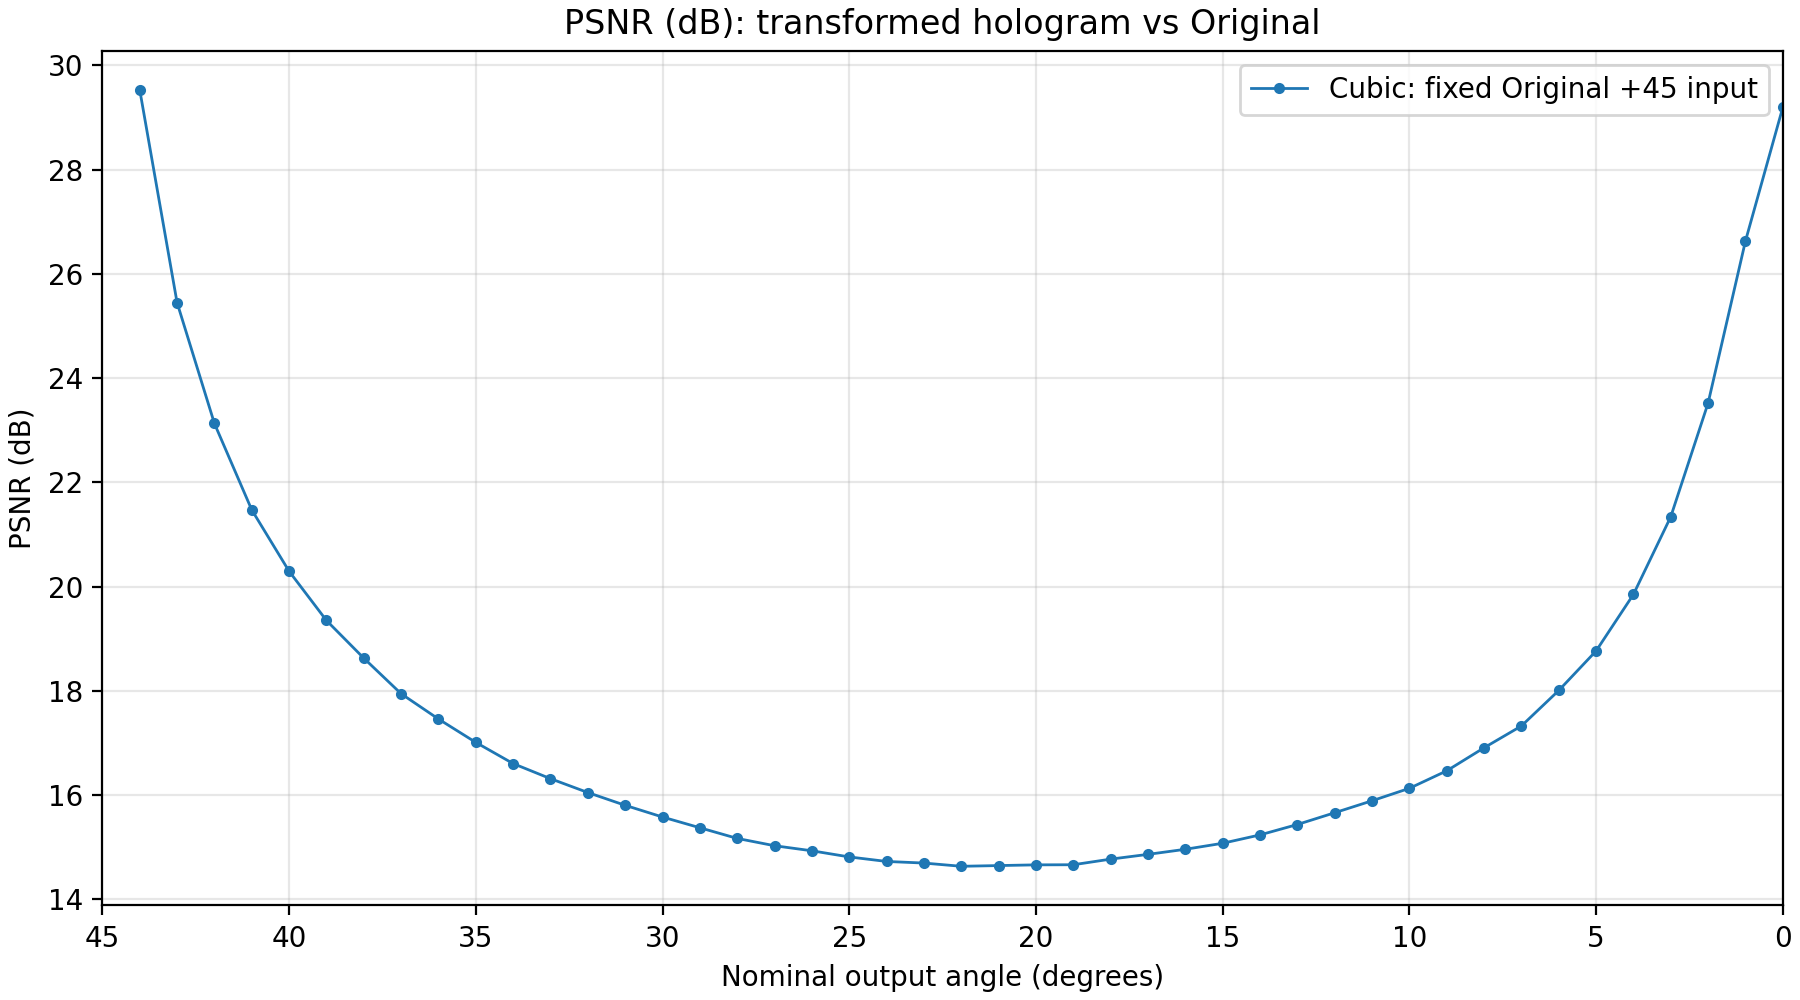
\includegraphics[width=.80\linewidth]{figures/psnr.png}
\caption{公称出力角度に対するPSNR。横軸は44度から0度へ進む。}
\end{figure}
\begin{figure}[H]\centering
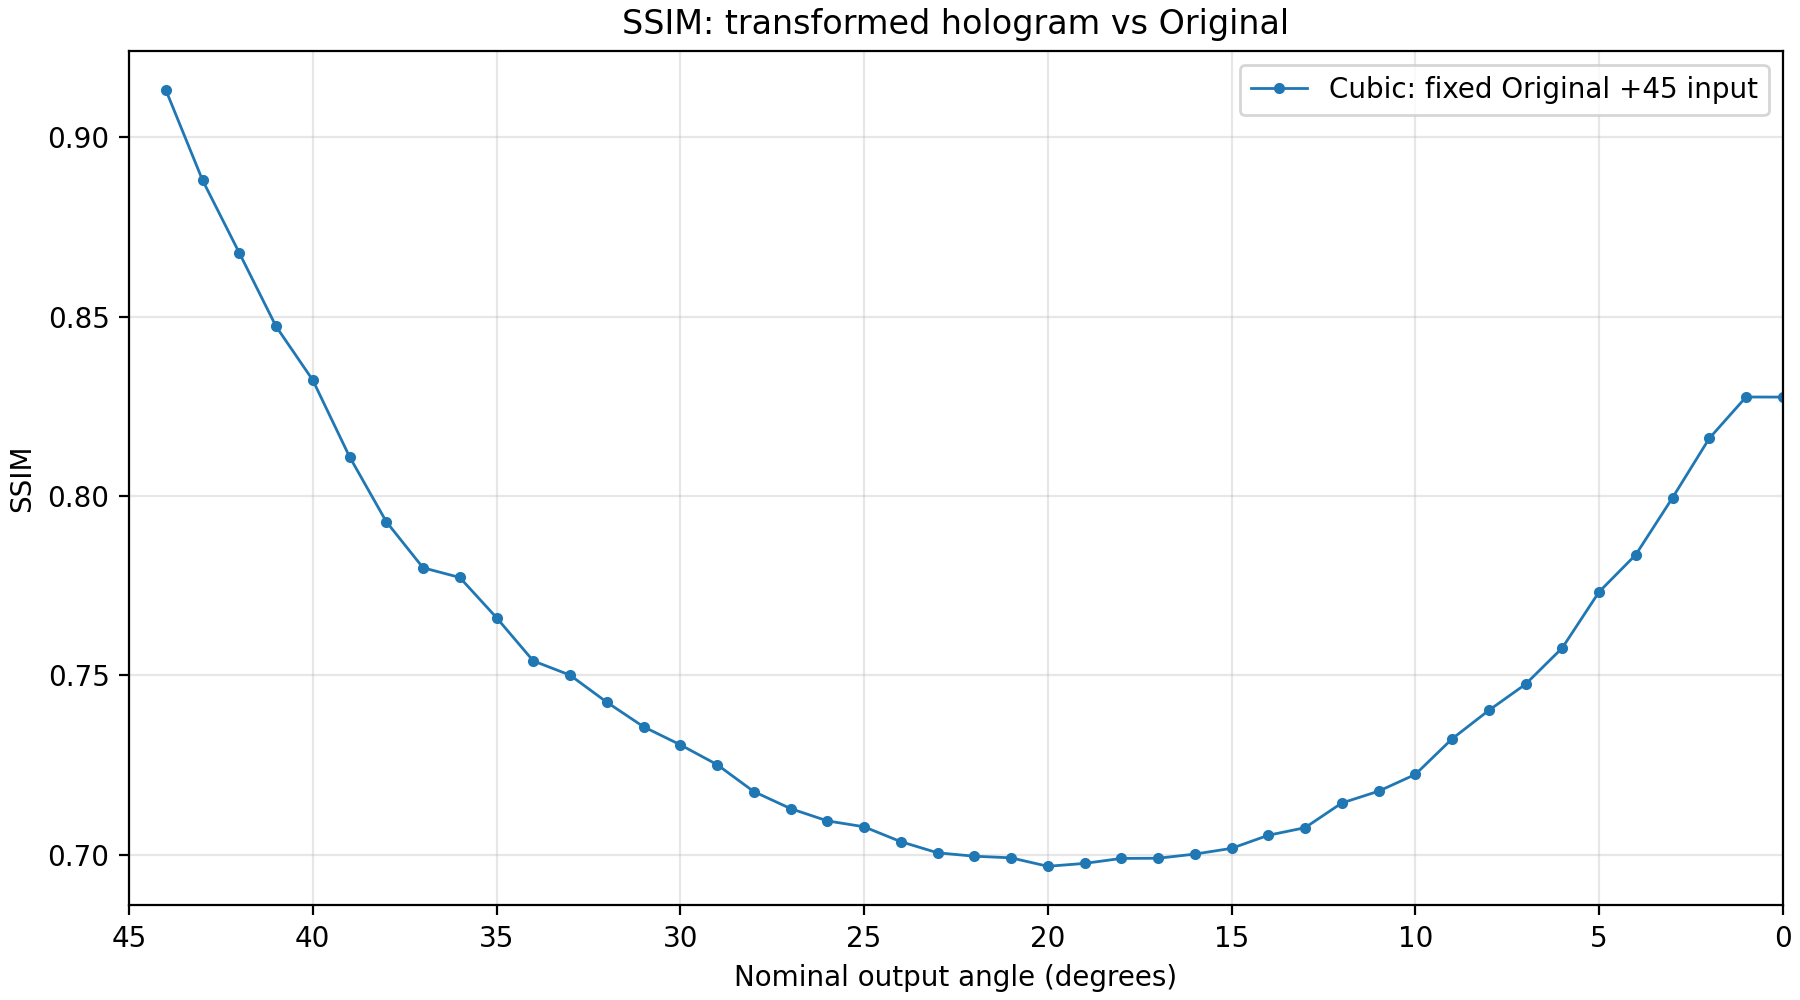
\includegraphics[width=.80\linewidth]{figures/ssim.png}
\caption{公称出力角度に対するSSIM。Original 45度を毎回入力とした独立変換の結果。}
\end{figure}
全45条件のPSNR平均は17.7766 dB、範囲は14.6330--29.5302 dB、
SSIM平均は0.7540、範囲は0.6967--0.9132であった。
両指標は出力角度20度前後で低く、0度付近で再び高くなる。
このため、今回の結果を単純な「回転量が増えるほど誤差が増える」とは説明できない。
連続変換ではないため、繰返し補間による誤差蓄積を測った結果でもない。

差の要因として、座標写像と回転方向の対応、有限標本・切出し、補間、
Original生成時の近軸近似と今回の平方根を用いた式の違いなどを切り分ける必要がある。
これらは現時点では候補であり、原因を特定した結果ではない。
また、本資料の平面間変換と、同じ観測面上で物体だけを回転させたOriginalどうしの関係は、
キャリアおよび伝搬条件を含めて別途確認する必要がある。
したがって、本実験は式の特殊ケースを実装し振幅の一致度を数値化した段階であり、
任意角度での幾何学的一致や複素波面の一致を実証したものではない。

\paragraph{再現用ファイル}
生成処理：\path{debug_code/generate_from_original45.py}。
評価処理：\path{debug_code/evaluate_from_original45.py}。
生成フォルダ内の\texttt{evaluation/psnr\_ssim\_results.csv}に全角度の数値、
\texttt{metadata.json}に生成条件を保存した。
\end{document}
